\documentclass[../main.tex]{subfiles}
\graphicspath{{\subfix{../assets/}}}

\begin{document}

\section{SUBLEQ}
\subsection{Limbaje ezoterice}
Limbajele de programare ezoterice se diferențiază față de cele obișnuite printr-o serie de factori, dar putem
spune că eficiența sau ușurința de a le folosi nu se află printre factori. \acrshort{intercal} \cite{intercal} 
este considerat primul limbaj ezoteric creat intenționat. În acest limbaj orice linie ce reprezintă o instrucțiune
validă poate contine cuvântul cheie \emph{``PLEASE''}. Compilatorul astfel se așteaptă la un anumit nivel de politețe
din partea programatorului. Dacă programul are prea puține sau prea multe apariții ale cuvântului \emph{``PLEASE''}
atunci compilatorul va arunca o eroare. Aproximativ între $1/5$ până la $1/3$ din instrucțiuni trebuie să fie
politicoase. Dacă o linie de cod nu este o instrucțiune validă atunci este ignorată. O metodă des întâlnită de a
lăsa comentarii este de a folosi \emph{``PLEASE NOTE''} urmat de textul comentariului. \emph{``NOTE''} nu este
o instrucțiune validă, motiv pentru care linia este ignorată, deci se comportă precum un comentariu.

Cele mai populare limbaje ezoterice sunt \emph{Brainfuck} \cite{brainfuck} și \emph{Befunge} \cite{befunge}.
\emph{Brainfuck} \cite{brainfuck} a fost inventa de către Urban Müller în 1993 într-o încercare de a scrie cel mai mic 
compilator pentru sistemul de operare AmigaOS versiunea 2.0, rezultatul a fost un compilator de 240B. Limbajul
consistă din o serie de comenzi ce servesc la manipularea unui vector de numere întregi, dimensiunea vectorului
nu este precizată în specificațiile limbajului și deci implementări diferite lucrează cu vectori de dimensiuni
diferite. \emph{Befunge} \cite{befunge} a fost inventat tot în 1993 de către Chris Pressey cu singurul scop de
a fi cât mai greu de compilat. Este un limbaj bi-dimensional, ceea ce înseamnă ca folosește un grid cu o dimensiune
fixă și ceea ce îl face greu de compilat este faptul că există comenzi ce modifică direcția de execuție a codului,
astfel codul poate fi executat din toate cele 4 direcții cardinale. Ambele limbaje consistă numai din comenzi de o 
singură literă, ceea ce face codul foarte greu de citit și de înteles, dând un nou înteles cuvântului \emph{obfuscat}.

Pe lângă cele menționate anterior există alte 2 limbaje care transcend timpul prin natura lor. Unul dintre ele
e un limbaj despre care se știe doar că niște călători în timp au confirmat existența lui cândva în viitor, cât
despre celălalt, are la bază doar conceptul de \emph{loop} ce nu poate fi terminat decât prin legarea lui la
durata de viață a unui număr sau concept pe care limbajul îl întelege. În teorie prin legarea unui \emph{loop} la univers,
acesta s-ar termina odată cu moartea universului. Folosind comanda \emph{EXECUTE} limbajul poate fi folosit pentru a
executa virtual orice, însă comanda poate fi folosită doar la finalul unui \emph{loop}, ceea ce poate presupune
așteptarea unei perioade lungi de timp.

Această secțiune servește drept introducere în minunata lume ezoterică a programării. Pentru mai multe detalii
vizitați \cite{esolangs}.

\subsection{OISC}
\emph{\acrfull{oisc}} sau \emph{\acrfull{urisc}} \cite{oisc} este o categorie de limbaje de programare ezoterice 
care au o singură instrucțiune, deși nu toate limbajele din acestă categorie sunt \emph{Turing complete} noi ne
vom axa pe cele care sunt. Există 3 subcategorii de limbaje \acrshort{oisc} \cite{oisc}:
\begin{itemize}
    \item \emph{\acrlong{tta}}
    \item \emph{Bit-manipulating machines}
    \item \emph{Arithmetic-based Turing-complete machines}
\end{itemize}

\emph{\textbf{\acrfull{tta}}} e un design în care operațiile de calcul sunt efecte secundare a unui transport de memorie.
De obicei niște regiștrii de memorie au o operație atribuită pe care o execută atunci când o operație de scriere
are loc asupra registrului. De exemplu, într-un \acrshort{oisc} care folosește o instrucțiune de copiere a unei valori
dintr-o locație de memorie în alta, poate fi implementat prin declanșarea unor regiștrii ce conțin operații aritmetice
și instrucțiuni de salt. Deși se utilizează o singură instrucțiune, este necesară implementarea \emph{hardware} a 
operațiilor ce se vor a fi executate, listă care poate conține orice număr arbitrar de operații.

\emph{\textbf{Bit-manipulating machines}} este cea mai simplă clasă, aceste limbaje se folosesc de operații logice pe biți
sau manipularea memoriei la nivel de bit. Exemple:
\begin{itemize}
    \item \emph{FlipJump} \cite{flipjump} este probabil cel mai simplu \acrshort{oisc} \cite{oisc}. Arată cu succes că
    ai nevoie de aproape nimic pentru a putea face orice. Are o singură instrucțiune cu 2 parametrii $A$ și $B$, adrese către un
    bit din memorie. Bitul care se află la adresa $A$ este negat, apoi execuția sare necondiționat la adresa $B$, echivalent cu:
    \begin{center}\ttfamily
        *A = !(*A);\\
        JUMP B;
    \end{center}
    \item \emph{BitBitJump} \cite{bitbitjump} perminte copierea unui bit dintr-o locație de memorie în altă locație de memorie,
    urmat de un salt necondiționat la o altă adresă. Se pare că acest proces este capabil de a executa orice operație, deoarece
    prin copierea biților se poate modifica codul ce urmează a fi executat. Instrucțiunea are 3 parametrii și se comportă astfel:
    \begin{center}\ttfamily
        *A = *B;\\
        JUMP C;
    \end{center}
    \item \emph{\acrshort{toga}} \cite{toga} este un alt limbaj care are o singură instrucțiune cu 2 parametrii. Numele vine de la \acrlong{toga}.
    Particular pentru acest limbaj este separamea memoriei de date și memoriei de program. Din cauza acestui amănunt nu este
    \emph{Turing complete}. Instrucțiunea se traduce în acest fel:
    \begin{center}\ttfamily
        MEMD[A] = !MEMD[A];\\
        IF (MEMD[A]) JUMP MEMP[B];
    \end{center}
\end{itemize}

\emph{\textbf{Arithmetic based Turing-complete Machines}} folosesc o operatie aritmetică și salt condiționat de rezultatul operației.
În comparație cu celelalte 2 clase \acrshort{oisc}, aceasta este \emph{Turing complete} prin natura ei. Instrucțiunile operează
cu numere întregi, care pot fi și adrese de memorie. Există o mulțime foarte mare de instrucțiuni în această subcategorie. Căteva exemple sunt:
\begin{itemize}
    \item \emph{\acrshort{addleq}} \cite{addleq} folosește operația de adunare:
    \begin{center}\ttfamily
        *B = *B + *A;\\
        IF (*B <= 0) JUMP C;
    \end{center}
    \item \emph{\acrshort{djn}} \cite{djn} folosește operația de decrementare:
    \begin{center}\ttfamily
        *A = *A - 1;\\
        IF (*A != 0) JUMP B;
    \end{center}
    \item \emph{\acrshort{p1eq}} \cite{p1eq} folosește operația de incrementare:
    \begin{center}\ttfamily
        IF (*A + 1 = *B) JUMP C;\\
        *B = *A + 1;
    \end{center}
    \item \emph{\acrshort{subleq}} \cite{subleq} folosește operația de scădere:
    \begin{center}\ttfamily
        *B = *B - *A;\\
        IF (*B <= 0) JUMP C;
    \end{center}
    \item \emph{Cryptoleq} \cite{cryptoleq} operează peste programe criptate:
    \begin{center}\ttfamily
        *B = $O_{1}$(*B, *A);\\
        IF ($O_{2}$(*B) <= 0) JUMP C;
    \end{center}
    Operațiile $O_{1}$ și $O_{2}$ sunt definite în lucrarea \cite{encript_comp} astfel:
    \begin{equation*}
        O_{1}(x, y) = x^{-1} \cdot y\;\mathrm{mod}\; N^{2},
    \end{equation*}
    \begin{equation*}
        O_{2}(x) = \left[\frac{x-1}{N}\right].
    \end{equation*}
    \item \emph{\acrshort{subleq}+} este o versiune a lui \acrshort{subleq} \cite{subleq} care folosește numere
    negative pentru adresare indirectă a memoriei. Se presupune că această variantă este \emph{Turing complete} și fără
    a folosi cod ce se modifică la execuție dar nu a fost demonstrat încă.
\end{itemize}

\section{Assembler}
\subsection{\emph{Two-Pass Assembler}}
Un \emph{assempler} este un program care traduce cod sursă, scris într-un limbaj de programare simbolic, în cod mașină,
instrucțiune cu instrucțiune. Codul mașină poate fi după încărcat în memorie pentru a fi executat de către dispozitivul
în cauză. Un \emph{assembler} poate, și face mai mult de atât, ajută programatorul în mai multe aspecte ale scrierii
programului.

Există mai multe tipuri de astfel de \emph{traducătoare} dar în mare putem vorbi despre \emph{one-pass assembler} și
\emph{two-pass assembler}. \emph{One-pass assembler} citește fișierul sursă, care conține codul ce se dorește a fi
tradus, o singură dată în timp ce \emph{two-pass assembler} citește fișierul sursă de 2 ori și de fiecare dată face
ceva diferit. În continuare ne interesează doar a doua categorie. Un \emph{assembler} cu un singur pass are mai multe
limitări care nu vor fi menționate aici dar le puteți găsi aici \cite{asl}. În figura \ref{fig:assembler} se poate 
vedea schema generală a unui \emph{assembler}.

\begin{figure}[h]
    \centering
    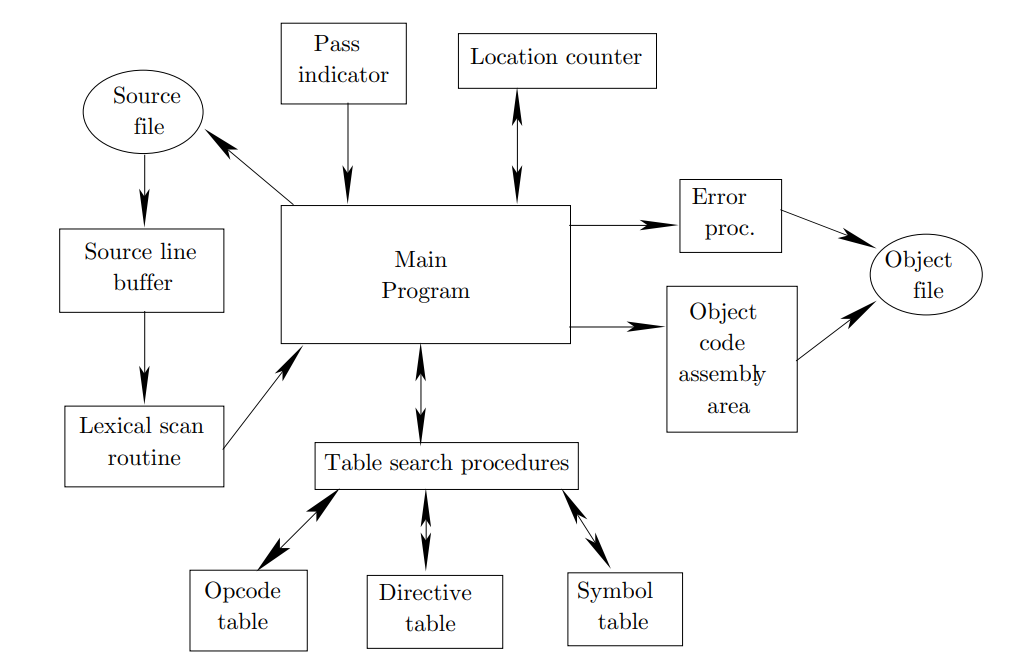
\includegraphics[width=0.8\textwidth]{assembler.png}
    \caption{Componentele principale ale unui \emph{assembler} extrasă din \cite{asl}}
    \label{fig:assembler}
\end{figure}

În primul pas citește fișierul sursă și caută toate \emph{etichetele}. O etichetă este doar un nume format din caractere
atribuit unei locații de memorie. Sunt foarte folositoare deoarece oamenii lucrează mai greu cu numere. O etichetă poate
fi folosită pentru a da un nume unei variabile, constante, locație în cod unde se află o instrucțiune, funcții, MACRO
și în funcție de limbaj pot fi și altele. În primul pas nicio instrucțiune nu este tradusă și toate etichetele sunt
salvate într-un tabel pentru a fi folosite în pasul următor. Pentru a putea atribui unei etichete valoarea corectă,
adică adresa corectă pe care o reprezintă, \emph{assembler}-ul trebuie totuși să interpreteze fiecare instrucțiune.
Acest lucru e necesar pentru că diferite instrucțiuni ocupă mai mulți \emph{bytes} în memorie în funcție de numărul
parametrilor dar și dimensiunea acestora.De asemenea unele directive se traduc în instrucțiuni sau date care sunt scrise
în memorie. În figura \ref{fig:first_pass} se vede ce se întămplă în pasul 1.
De cele mai multe ori, dar nu e o regulă generală, la acest pas se construiește un fișier intermediar ce
contine codul din fișierul sursă împreună cu informațiile culese și prelucrate în acest pas pentru a fi transmise la
pasul 2.

\begin{figure}[h]
    \centering
    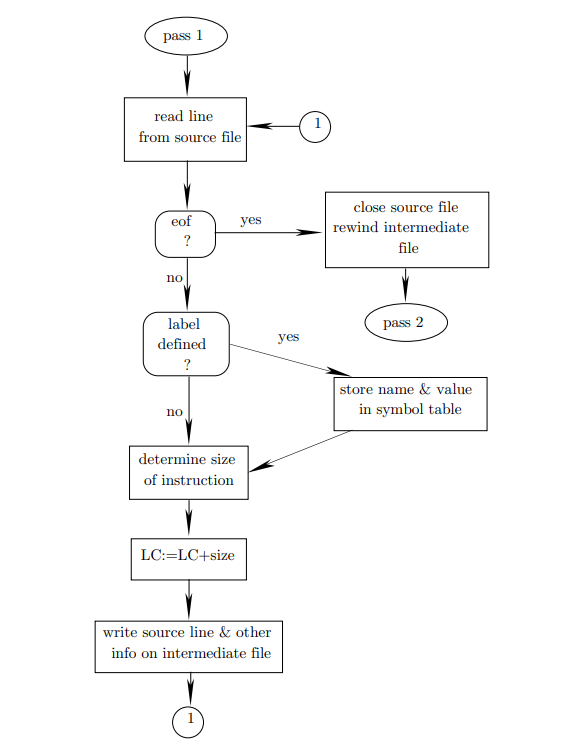
\includegraphics[width=0.8\textwidth]{first_pass.png}
    \caption{Primul pas extrasă din \cite{cache}}
    \label{fig:first_pass}
\end{figure}

Pot să apară 3 probleme cu etichetele la pasul 1. Etichetele pot fi definite în mai multe locuri, numele unei etichete
nu respectă regulile limbajului și etichete nedefinite dar utilizate. Dacă o etichetă este definită în mai multe locuri
atunci cum se decide care este valoare ei? O etichetă ar trebui să fie un nume unic atribuit unei adrese pentru a putea
fi ușor de folosit în cod. Multe limbaje nu permit simboluri speciale în numele etichetelor, de obicei sunt permise
caracterele alfanumerice și bară orizontală `\_' dar primul caracter nu poate fi o cifră. O etichetă este nedefintă dacă
este folosită în cod fără a fi definită, deci nu are o valoare atribuită.

Pasul al 2-lea se ocupă cu traducerea instrucțiunilor în cod mașină. La fel ca la pasul anterior citește
fișierul intermediar și interpretează fiecare instrucțiune apoi o scrie în fișierul final. Când întâlnește
o etichetă o înlocuiește cu valoarea ei. În figura \ref{fig:second_pass} se vede ce se întămplă în pasul 2.

\begin{figure}[h]
    \centering
    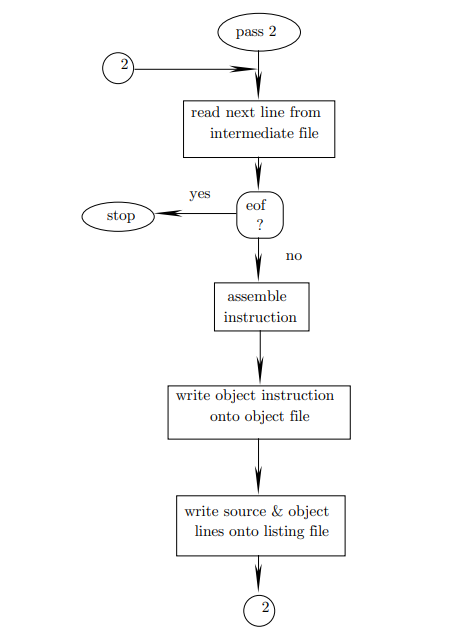
\includegraphics[width=0.8\textwidth]{second_pass.png}
    \caption{Al doilea pas extrasă din \cite{asl}}
    \label{fig:second_pass}
\end{figure}

\clearpage
\subsection{Directive}
Aici începe frumusețea unui \emph{assembler} dar nu aici se și termină. Pe lângă instrucțiuni un \emph{assembler} oferă
și directive, acestea sunt comenzi suplimentare care sunt executate sau interpretate de către \emph{assembler} dar nu 
sunt traduse. Unele directive ar putea fi interpretate în instrucțiuni și apoi traduse dar directiva în sine nu e
specifică limbajului. Pot fi împărțite pe categorii funcționale. Capitolul 3 din \cite{asl} este dedicat directivelor.

\subsection{MACRO}
În sine macro-urile sunt de asemenea directive dar pentru că sunt foarte folosite sunt considerate ca fiind ceva diferit
și de sine stătător. Un macro e similar cu o subrutină dar există o diferență majoră între cele 2. O subrutină este o
bucată de cod care e scrisă o singură dată și apoi poate fi folosită oriunde în cod prin simpla apelare. Un macro este
tot o bucată de cod care e definit o singură dată și poate fi folosit de mai multe ori în cod dar de fiecare dată codul
este copiat pur și simplu. Prin urmare subrutinele sunt tratate de către \emph{hardware} la execuție, iar macro sunt
tratate de \emph{assembler} la compilare/asamblare/traducere. Pasul 0 este un pass special care e responsabil de a interpreta
toate macro-urile și de a le expanda unde sunt folosite. Capitolul 4 din \cite{asl} este dedicat macro-urilor.

\subsection{Analiză lexicală}
În implementarea unui \emph{assembler} analiza lexicală este primul și cel mai important proces. Un \emph{assembler}
lucrează cu fișiere text, fișierul sursă și cele intermediare. Un calculator lucrează cu codul mașină, el cunoaște doar
0 și 1 dar pentru oameni nu e deloc intuitiv, din cauza asta trebuie să lucrăm cu fișiere text care sunt usor de citit
și de scris pentru noi. Analiza lexicală este primul proces care are loc în care codul sursă este transformat într-un 
șir de simboluri. Aceste simboluri sunt definite în funcție de nevoile limbajului, astfel încât să acopere toate
elementele din cod. Exemplul următor explică aplicarea analizei lexicale asupra unei linii de cod dintr-un limbaj
de programare arbitrar de nivel înalt:

{\ttfamily
    \begin{verbatim}
int x = (a + b) * 2;

KEYWORD int
IDENTIFIER x
EQUALS
OPEN_PARANTHESIS
IDENTIFIER a
PLUS
IDENTIFIER b
CLOSE_PARANTHESIS
TIMES
LITERAL 2
SEMICOLON
    \end{verbatim}
}

Mai departe se trece la validarea sintaxei, o altă parte a analizei lexicale. Considerând exemplul anterior, trebuie să
validăm că o paranteză deshisă este și închisă, dupa `=' trebuie să urmeze o expresie validă, ultimul simbol trebuie să
fie \texttt{SEMICOLON}, după `int' trebuie să urmeze un identificator, etc. În final simbolurile trebuie stocate și trimise
către următorul proces împreună cu erorile găsite, după cum se vede în figura \ref{fig:lexer}. Pentru explicații mai
detaliate continuați cu \cite{lexer}.

\begin{figure}[h]
    \centering
    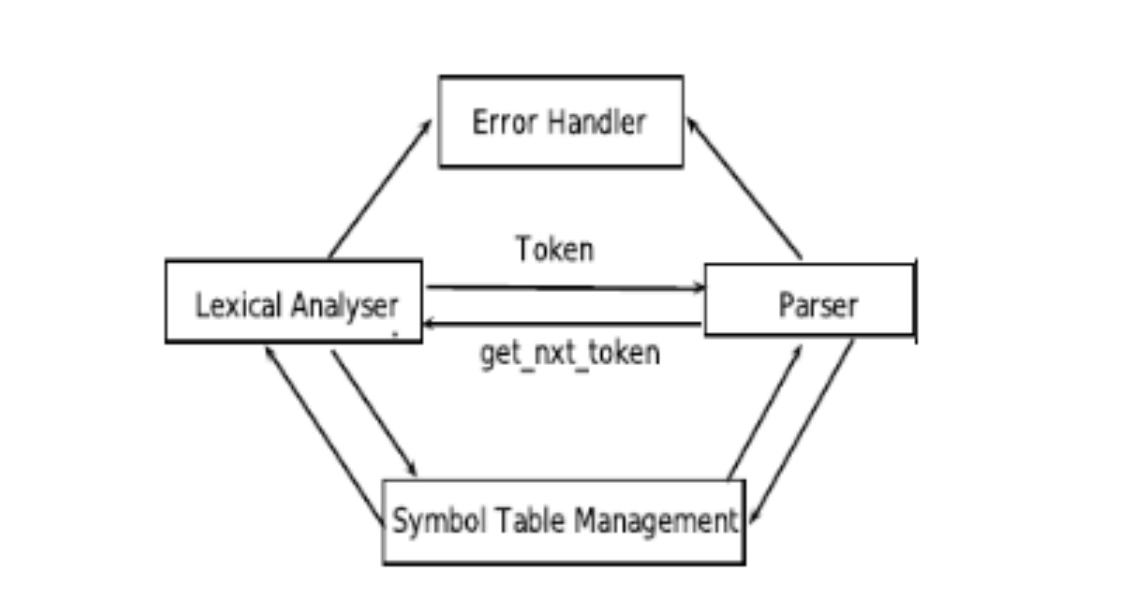
\includegraphics[width=0.8\textwidth]{lexer.png}
    \caption{Analiză lexicală extrasă din \cite{lexer}}
    \label{fig:lexer}
\end{figure}

\section{Procesor}
\subsection{Automat cu stări finite}
Procesorul este creierul unui calculator, cel care coordonează celelalte \emph{organe} și ia decizii. Presupun că sursa
de alimentare e inima atunci. Procesoarele care există azi sunt extrem de complexe, fie că sunt \acrfull{cisc} sau
\acrfull{risc} tot au sute de instructiuni diferite \cite{intel64}. Am obosit. Procesorul citește instrucțiuni din memorie,
pe care le execută și enentual scrie înapoi în memorie. Deja avem un instrument foarte puternic dar nu e foarte util
până nu introducem operații de intrare ieșire pentru a avea control asupra a ce se executa, cum și cănd.

Un automat cu stări finite e o mașina abstractă care se află în exact o stare din mulțimea stărilor în care se poate afla.
Poate trece dintr-o stare în alta în mod necondționat sau condiționat de anumite date de intrare. Trecerea dintr-o stare
în alta se numește tranziție. Și atunci un automat cu stări finite este definit de mulțimea stărilor, stare inițială în care
se află, tranzițiile și ce date de intrare declanșează tranzițiile. Multe dispozitive automate nu au nevoie de circuite
complexe pentru a opera. O ușă care se deschide automat poate fi implementată ca un automat cu stări finite cu 4 stări
\texttt{(CLOSED, OPENING, OPEN, CLOSING)}, iar ca date de intrare are un semnal de un bit, 1 dacă senzorul de greutate
e apăsat, 0 dacă nu e.

Procesoarele foarte simple pot fi implementate ca automate cu stări finite, precum în figura \ref{fig:fsm}.

\begin{figure}[h]
    \centering
    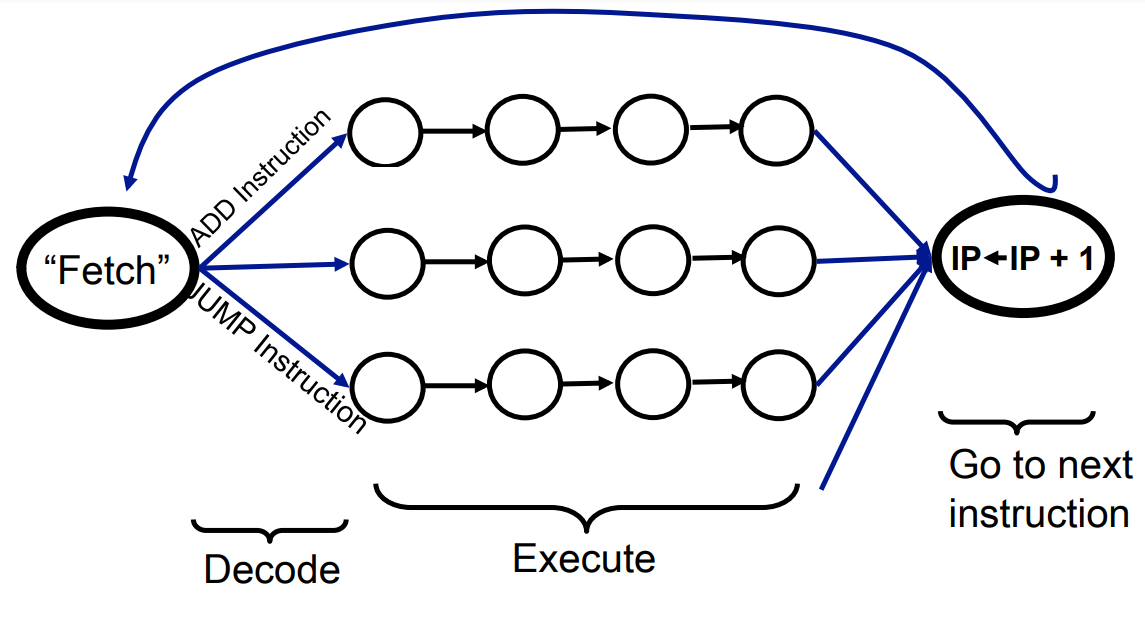
\includegraphics[width=0.8\textwidth]{fsm.png}
    \caption{Procesor ca automat cu stări finite din \cite{fsm}}
    \label{fig:fsm}
\end{figure}

\subsection{Memoria cache}
Prin memorie definim un dispozitiv de stocare a informației. Memoriile pot fi de foarte multe tipuri și pe multe categorii.
Avem memorii volatile și nevolatile, după durata de viață a informației. Volatil inseamnă că în momentul în care sursa
ce alimentează dispozitivul e oprită informația se șterge, e nevoie de un efort/energie pentru a menține starea memoriei.
Memoriile nevolatile consumă energie la citire și scriere și păstrează permanent informația, cel puțin în teorie, din păcate
totul e afectat de entropie. O altă categorie e dimensiunea spațiului de stocare și viteza de răspuns. Le luăm Impreună
deoarece viteza de răspuns e în general invers proporțională cu dimensiunea spațiului de stocare. De asemenea viteza de
răspuns crește cu cât distanța fizică dintre memorie și alt dispozitiv ce accesează memoria este mai mică. În figura
\ref{fig:memory_pyramid} se poate observa ierarhia acestei categorii.

\begin{figure}[h]
    \centering
    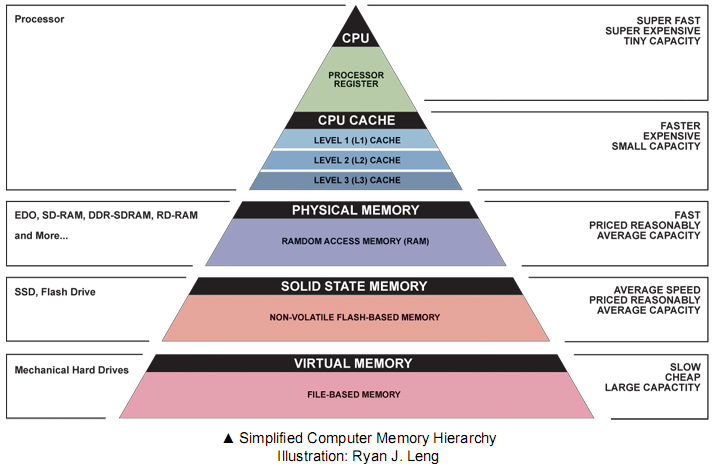
\includegraphics[width=0.8\textwidth]{memory_pyramid.png}
    \caption{Ierarhia tipurilor de memorie din \cite{memoryhierarchy}}
    \label{fig:memory_pyramid}
\end{figure}

În figura \ref{fig:memory_pyramid} nu apare cea mai de jos categorie, care este \emph{Harder Drive} \cite{harderdrive}. 
Am vorbit despre limbaje de programare ezoterice \cite{esolangs}, \emph{Harder Drive} \cite{harderdrive} e cam același 
lucru dar pentru spații de stocare a informației. Cele 3 exemple de implementări date în \cite{harderdrive} sunt:
\begin{itemize}
    \item \acrshort{icmp} ECHO sau PING în varianta cu \emph{payload}
    \item Jocul TETRIS în care fiecare bloc ocupat înseamnă 1, altfel 0
    \item Teste COVID-19 electronice folosite, puse pe o placă PCB
\end{itemize}

Dacă ne întoarcem atenția către memoria cache, observăm că există mai multe niveluri pe care e distribuită. Memoria cache
de nivel 1 este cea mai aproape de procesor și în cazul unui procesor multi-core nu e împărțiță, fiecare core are câte un
cache L1. Nivelul 2 în acest caz este pentru perechi de core-uri, dar nu e neapărat să fie pentru fiecare 2, poate fi pentru
fiecare 3 sau 4 sau mai multe core-uri, după caz. Nivelul 3 e cel mai mare, inclusiv la spațiu și la el au acces toate
core-urile. Ierarhia aceasta există tocmai pentru a evita situația în care va trebui ca date sau instrucțiuni să fie încărcate
din memoria RAM care e prea lentă ca să țină pasul cu procesorul, după cum e descris în \cite{bottleneck} unde sunt prezentate 
și alte soluții la această problemă.

Există mai multe tipuri de memorie cache. Se caracterizează prin comportamentul lor atunci când apare un cache miss la scriere
sau la citire dar și după organizarea blocurilor de memorie. După organizarea blocurilor de memorie distingem cache cu
mapare directă, total asciativă sau asociativă pe seturi. Maparea decide în ce linie din cache poate un bloc de la o anumită 
adresă să fie stocat. Politica de înlocuire decide ce linie va fi înlocuită în cazul unui \emph{cache miss}, depinde de
mapare, în cazul mapării directe un bloc de memorie poate fi pus într-o singură linie deci nu e nevoie de politică de
înlocuire. Sunt 2 tipuri de strategii de scriere \emph{write through}, informația e scrisă atât în cache cât și în memoria RAM
și \emph{write back}, informația e scrisă doar în cache, urmează să fie scrisă în memorie cănd linia e înlocuită. În cazul unui
\emph{cache miss} la scriere blocul poate fi încărcat în cache \emph{write allocate} sau nu \emph{no-write allocate}
\cite{cache}.

\subsection{Sincronizarea circuitelor cu frecvențe diferite}
Dacă nu ești tu inginerul care se ocupă de realizarea tuturor componentelor unui sistem atunci cel mai probabil nu toate
au aceeași frecvență de operare. Chiar dacă ești, tot pot să existe motive pentru care asta se întâmplă, cum ar fi
limitări fizice, reducerea costului sau reducerea consumului de energie, etc. Apare problema de comunicare sincronizată
între 2 circuite. O soluție la această problemă este \emph{hanshacking}, folosită de altfel și la rețele în protocolul
\acrshort{tcp}. Implementarea circuitului de sincronizare este redată în figura \ref{fig:handshake} și modul de funcționare
în figura \ref{fig:handshake_rules}. Mai multe soluții găsiți aici \cite{sync}.
Alte soluții precum \emph{clock domain crossing} sunt amintite și aici \cite{block_memory}.

\begin{figure}[h]
    \centering
    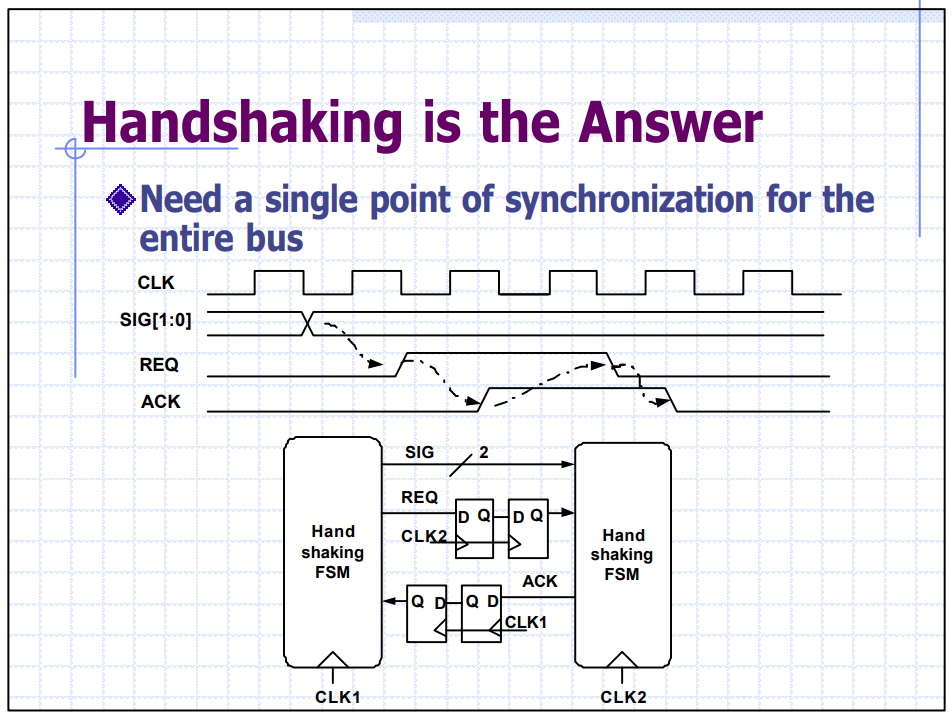
\includegraphics[width=0.8\textwidth]{handshake.png}
    \caption{Sincronizare prin \emph{handshaking} din \cite{sync}}
    \label{fig:handshake}
\end{figure}

\begin{figure}[h]
    \centering
    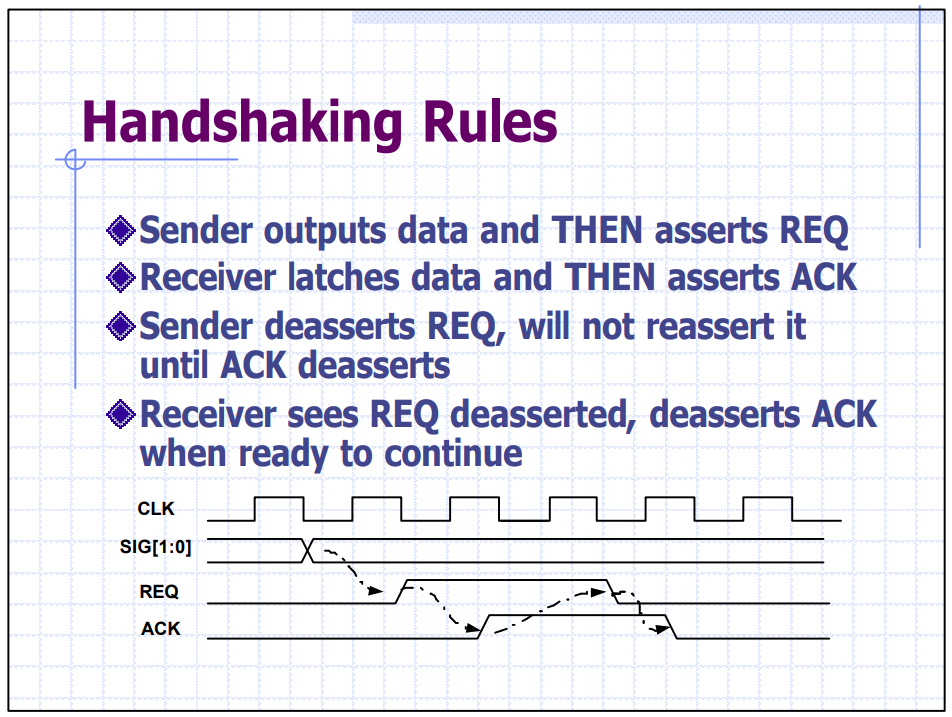
\includegraphics[width=0.8\textwidth]{sync_rules.png}
    \caption{Sincronizare prin \emph{handshaking} din \cite{sync}}
    \label{fig:handshake_rules}
\end{figure}

\end{document}